\documentclass[a4paper, 12pt, twoside, openright]{mythesis}

\include{macros}

\renewcommand{\baselinestretch}{1.5}

%\hypersetup{
%    colorlinks=true,       % false: boxed links; true: colored links
%    linkcolor=blue,          % color of internal links
%    citecolor=blue,        % color of links to bibliography
%    filecolor=blue,      % color of file links
%    urlcolor=blue           % color of external links
%}

%------------------------------------
% Thesis boundary Setting
%-------------------------------------

\textwidth      = 137.0mm
\textheight     = 224.0mm
\topmargin      =  -3.0mm
\headheight     =   7.0mm
\headsep        =  10.0mm
\footskip       =   8.0mm
\oddsidemargin  =  10.6mm
\evensidemargin =  10.6mm
\hoffset = -0.2cm
%\overfullrule=5pt%%

\pagenumbering{roman}% \thispagestyle{myheadings}
\setcounter{page}{1}
%\thispagestyle{empty}

\begin{document}
\title{\textbf{Model-free Iterative Learning Control with Recursive Convergence Acceleration for Tracking Control Application}}


\author{ \\  \\ \\
{\it Gen-Hao Zhang}\\
{\it Advisor: Shao-Yi Chien} \\ \\ \\ \\  \\ \\
{\it Graduate Institute of Electronics Engineering}\\
{\it National Taiwan University} \\
{\it Taipei, Taiwan}\\ }

{\date{May 2020}}

\maketitle

\frontmatter
\input{inc/0_abstract/abstract.tex}
\tableofcontents
\listoffigures
\listoftables

%------------------------------------
% Thesis Body -- begin
%------------------------------------

\mainmatter





%------------------------------------
% Chapter 1 
%------------------------------------



\chapter{Introduction}
\label{ch:intro}

\section{Motivation}
\label{sec:Motivation}



Tracking control problem, which is to make a physical system to move along a desired time-dependent trajectory, has been a critical issue in control applications for many years \cite{tomizuka1987zero}. For example, for a CNC machine, each axis has to follow the position command signal produced by the trajectory interpolator  \cite{ramesh2005tracking}. Traditionally, the tracking control problem is solved by closed-loop feedback control structure, as shown in Fig. \ref{fig:FB_Ctrl}, where $P(z)$ is the physical system to be controlled (usually called "plant"), $u(k)$ is the control input signal of $P(z)$, $y(k)$ is the output signal of $P(z)$, and $r(k)$ is the desired reference signal that $P(z)$ to be followed. Note that $k$ is the discrete time index of the signal, and $z$ is the delay operator for a system represented in z-domain transfer function form. For this structure, to let the system output $y(k)$ track along the desired reference signal $r(k)$, the controller $C(z)$ is introduced to minimize the tracking error $e(k):= r(k)-y(k)$. Therefore, the tracking control problem can be stated as the following optimization goal:


\begin{equation}
\min_{C(z)} \left \| r(k)-y(k) \right \|_2
\label{eq:TrackingCtrl_Prob}
\end{equation}



\begin{figure}
 	\begin{center}
   	\includegraphics[width=1.1\linewidth] {image/FB_Ctrl}
 	\caption{The structure of feedback control system.}
 	\label{fig:FB_Ctrl}
 	\end{center}
\end{figure}

To implement the controller $C(z)$, which is a causal and LTI digital filter, the computation from $e(k)$ to $u(k)$ is usually done by a real-time program in microcomputer. Specially, proportional-integral-derivative(PID) controller is the most common used ones in industry applications  \cite{ramesh2005tracking}. For PID-based feedback control approach, the pseudo code of the real-time control can be written as:

\begin{algorithm}[htbp]
 \caption{PID-based Feedback Control}
  \label{alg:PID}
  \begin{algorithmic}[1]
    \Require The desired reference trajectory $r(k)$ with length $N$.
    \Ensure The control input $u_{k}$ 
    \State Initialize the last error $e_{k-1} \gets 0$;
    \State Initialize the error summation $e_{\Sigma} \gets 0$;
    \For{$k=1$ to $N$}
    
     \State measure the current output signal $y_{k}$;
     \State compute the current tracking error: $e_{k}=r[k]-y_{k}$;
     \State PID control law: $u_{k}=k_{p}e_{k}+k_{I}e_{\Sigma}+k_D(e_{k}-e_{k-1})$; $//C(z)$
     \State send the control input signal $u_{k}$ to the system;
     \State record the last error $e_{k-1} \gets e_{k}$;
     \State compute the error summation $e_{\Sigma} \gets e_{\Sigma}+e_{k}$;
    \EndFor
	
	\State Note: The for-loop conducts for 1 sampling period for each loop.
  \end{algorithmic}
\end{algorithm}

The advantages of PID-based feedback control are simple, easy-to-implement and model-free, which only need to tune PID parameters $k_{P}$, $k_{D}$ and $k_{I}$ without knowing the plant model $P(z)$ in advance, hence it is widely used in industry applications. From the pseudo code of the feedback control algorithm, we can observe that once the tracking error occurs, controller $C(z)$ reacts to the error to compute a suitable control input $u$ to remedy the output result. However, this property results the lag in transient tracking, hence the tracking performance of PID-based feedback control algorithm is limited since the feedback controller $C(z)$ only takes action if the error is not zero \cite{ oomen2020learning}.


\begin{figure}
 	\begin{center}
   	\includegraphics[width=1\linewidth] {image/FF_Ctrl}
 	\caption{The structure of feedforward control system. $F(z)$ is the feedforward compemsator of the closed-loop system $G(z)$, and the optimal design of $F(z)$ is $F(z)=G^{-1}(z)$, which make the overall system $\frac{Y}{R}:=F(z)G(z)=1$ if the disturbance $d(k)$ is not considered.}
 	\label{fig:FF_Ctrl}
 	\end{center}
\end{figure}


\begin{figure}
 	\begin{center}
   	\includegraphics[width=1.1\linewidth] {image/Repetitive}
 	\caption{The structure of repetitive control system. $F(z)$ is the inversion-based filter of the stable system $G(z)$. The stability condition of RC is $\left \| I-Q(z)F(z)G(z) \right \|_\infty<1$, where $Q(z)$ is a zero-phase low pass filter, hence the optimal design of the $F(z)$ is $F(z)=G^{-1}(z)$.}
 	\label{fig:RC}
 	\end{center}
\end{figure}


\begin{figure}
 	\begin{center}
   	\includegraphics[width=1.1\linewidth] {image/ILC}
 	\caption{The control architecture of iterative learning control. $L(z)$ is the learning filter of ILC and $G(z)$ is a stable system. The stability condition of ILC is $\left \| I-L(z)G(z) \right \|_\infty<1$, hence the optimal design of the $L(z)$ is $L(z)=F(z)=G^{-1}(z)$.}
 	\label{fig:ILC}
 	\end{center}
\end{figure}

To remedy the difficulty that feedback control approach faced, several methods has been proposed, such as feed-forward control[], iterative learning control[] and repetitive control[]. For these approaches, the inversion-based compensator $F(z)$ plays the most important role in the tracking performance, and the optimal design of $F(z)$ is:

\begin{equation}
 F(z) = G^{-1}(z)
\label{eq:F(z)}
\end{equation}
 
\begin{equation}
 G(z) =\frac{C(z)P(z)}{1+C(z)P(z)}
\label{eq:Closed_loop_G(z)}
\end{equation}
 
where $F(z)$ is the inversion-based compensator $($also called feedforward compensator, inversion-based filter, and inversion-based learning filter in feedforward control, repetitive control and iterative learning control $)$, and $G(z)$ is a SISO, LTI and stable system that can be stabilized by the feedback controller $C(z)$.



The motivation of this thesis is to construct a novel algorithm and provide a systematic procedure to improve the performance of each advanced control method mentioned above. Specially, we focus on the development of a model-free iterative learning control algorithm. Our algorithm not only improves the tracking performance of that feedback control, but also 




To construct the optimal compensator $F(z)$ for feedforward control, iterative learning control and 
%Iterative learning control (ILC), which operates the same task repeatedly and updates the control input according to the previous trial data, has been applied in tracking control applications for many years [\cite{ahn2007iterative}]. Since the learning operation can be non-casual, ILC has been shown to achieve better tracking performance compared to feedback control approaches [\cite{bristow2006survey}]. 


%\subsection{Table}
%\label{sec:Table}
%The related information is shown in~\tabref{lab_information}.
%
%\begin{table}[p]
%\vergap{0.8}
%\horgap{4.5pt}
%\caption{Lab information.}
%\vspace{5pt}
%\label{tab:lab_information}
%\centering
%\footnotesize 
%\begin{tabular}{cc}
%\toprule
%Property & Description \\
%\midrule
%Professor & Shao-Yi Chien \\
%Labs & BL421, MD431, MD726 \\
%\bottomrule
%\end{tabular}
%\end{table}








\section{Previous Work and Problem Formulation}
\label{sec:Previous Work and Problem Formulation}

To reduce the tracking error iteratively, the ILC updating law has to be well designed. The model-based ILC [\cite{lee1994feedback}; \cite{harte2005discrete}] uses the system inverse model as the learning filter to conduct the learning process. For these approaches, if the system model is identified accurately, the learning process would converge within few iterations [\cite{teng2015comparison}]. However, inversion-based methods require delicate modeling process in advance, which isn't practical for industry applications. Due to the reasons mentioned above, the development of model-free ILC becomes more and more popular in the ILC research community \cite{janssens2011model}.

For the model-free approaches, the PD-type ILC [\cite{arimoto1984bettering}; \cite{chen2006pd}] is the simplest way to implement. However, monotonic convergence condition is not always satisfied by tuning the PD-parameters [\cite{moore2005monotonically}], and the tuning process may be time-consuming and damage the system. Time-reversal based ILC [\cite{ye2005zero}] uses the adjoint operator of the system as the learning filter, and the control updating law can be implemented by filtering the reversed error signals using the system itself. However, the learning rate of the time-reversal based ILC is usually slow [\cite{chen2017data}].  

To achieve a fast error convergence rate, the model-free inversion-based iterative learning control (MFIIC) [\cite{kim2012modeling}] applies the point-by-point division over the discrete frequency interval to estimate the system inverse dynamics from the input and output signals. Nevertheless, the output disturbances present in the denominator of the computation. Once unpredicted output disturbances are introduced, the magnitude of the denominator may approach to zero. This unpredicted phenomenon leads to a poor transient learning behavior [\cite{de2018improving}]. To improve the learning transient performance, NLIIC [\cite{de2019data}] uses an adaptive learning gain to avoid the division by a small numbers. However, since the adaptive learning gain shuts down the learning for the frequency components dominated by the output disturbances, the tracking performance in steady-state is degraded.      


\section{Proposed Approach and Contributions}
\label{sec:Proposed Approach and Contributions}

To overcome the difficulties mentioned above, a model-free learning algorithm is proposed. The proposed algorithm is based on the time-reversal based ILC, and we apply a data-based learning filter to update the control input every $n$ iterations. This approach not only accelerates the convergence rate of time-reversal based ILC. Compared to the MFIIC and NLIIC approaches, our method provides a more flexible updating law that gains the robustness against output disturbances and the tracking performance in steady-state.

\section{Thesis Overview}
\label{sec:Thesis Overview}

The remainder of this paper is organized as follows: Section 2 illustrates the basic iterative learning control algorithm and the existing model-free ILC approaches. Section 3 provides a derivation and analysis of the proposed model-free learning algorithm. Section 4 presents the simulation results to validate the effectiveness of the proposed algorithm. Finally, Section 5 summarizes the main results and contributions of this paper.


















%------------------------------------
% Chapter 2
%------------------------------------



















\chapter{Related Work}
\label{ch:related_work}

\section{Repetitive Control and ILC}
\label{sec: Repetitive Control and ILC}


\subsection{Repetitive Control}
\label{sec: Repetitive Control}

\subsection{Iterative Learning Control}
\label{sec: Iterative Learning Control}

  For a SISO, LTI system $G(z)$, which is represented in z-domain and assumed to be asymptotically stable, the ILC learning algorithm can be written in the following form:

\begin{align}
\begin{split}
u_{j+1}(k)& = u_j(k)+L(z)[r(k)-y_j(k)]\\
& = u_j(k)+L(z)e_j(k)
\end{split}
\label{eq:ILClaw}
\end{align}


where $k$ is the time index of the discrete-time signal, the sub-index $j$ represents the $j$th iteration of learning process, $r$ is the trial-invariant reference to be tracked with time interval $N$, $u$ represents the control input of $G(z)$, $y$ is the output of  $G(z)$, $e$ is the tracking error to be reduced, and $L(z)$ is the learning filter to guarantee the stable learning.
 
{$Assumption$ 1.}
Since the z-transform and Fourier transformation of a time sequence is computed over an infinite time interval, all the time signals in this paper are assumed to have infinite length (i.e. $N$$\rightarrow$$\infty$) to meet the requirement of frequency-domain analysis [\cite{silverman1973deconvolution}]. 

$Assumption$ 1 is necessary for ILC analysing in z-domain since the convolution theorem in z-domain is hold iff the time-sequences are all with infinite length.

To analysis the ILC stability condition in frequency domain, the error propagation formula can be obtained from Eq. \ref{eq:ILClaw}:
\begin{equation}
e_{j+1}(k)= [1-L(z)G(z)]e_j(k)
\label{eq:ILCerr}
\end{equation}

By taking Fourier transform of Eq. \ref{eq:ILCerr}, apparently, the tracking error will converge if:
\begin{equation}
\left \| I-G(z)L(z) \right \|_\infty<1
\label{eq:ILCstability}
\end{equation}
where $\left \| \cdot  \right \|_\infty$ denotes $\mathcal{H}_\infty$-norm. It had been proven when the learning filter $L(z)$ satisfies Eq.\ref{eq:ILCstability}, the control input $u_\infty$ and tracking error $e_\infty$ will converge and thus the learning is stable [\cite{norrlof2002time}] . 

{$Remark$ 1.}
To meet the infinite long time signal assumption, the zero-padding technique is applied to extend the reference signal with sufficient long zeros on the both ends to avoid leakage in frequency-domain computation.   


\subsection{Inverse Filter Design of RC and ILC}
\label{sec: Inverse Filter Design of RC and ILC}


\section{Inverse Filter Design Method for Repetitive Control and ILC}

\subsection{Zero Phase Error Tracking Control (ZPETC)}
\label{sec: Zero Phase Error Tracking Control (ZPETC)}

\subsection{Unity Magnitude Error Tracking Control (UMETC)}
\label{sec: Unity Magnitude Error Tracking Control (UMETC)}

\subsection{Direct Inversion Method}
\label{sec: Direct Inversion Method}

\subsection{Iterative Learning of Dynamic Inverse Filters (ILCFF)}
\label{sec: Iterative Learning of Dynamic Inverse Filters (ILCFF)}

\section{Model-free ILC}
\label{sec: Model-free ILC}
To satisfy the stability criteria and the model-free requirement, there are several ways to implement the model-free leaning law. Here the time-reversal based ILC and MFIIC approaches are introduced.



\subsection{Model-free Adjoint-based ILC}
\label{sec: Model-free Adjoint-based ILC}

Consider the adjoint-based ILC [\cite{ye2005zero}; \cite{owens2009robust}], the learning filter $L(z)=\alpha G^{*}(z)$ is chosen with a sufficiently small learning gain $\alpha>0$ to guarantee the stability condition. The reason why the adjoint-based learning filter is capable to stabilize the learning is the phase effect of the system could be cancelled, hence the stable learning can be hold if the learning gain is properly selected.

To realize the adjoint-based learning law:
\begin{equation}
u_{j+1}(k)= u_{j}(k)+ \alpha G^{*}(z)e_{j} (k)
\label{eq:TimeRever}
\end{equation}

the term $\alpha G^{*}(z)e_{j} (k)$ can be obtained by using the reversed time filtering technique as shown in [\cite{ye2005zero}]:

\begin{enumerate}
  \item Reverse the error signal: $e_{j1}(k)=e_{j}(N-k)$;
  \item Feed the reversed error signal to the system: $e_{j2}(k)=G(z)e_{j1}(k)$;
  \item Reverse $e_{j2}(k)$ again, and multiply with $\alpha$:  $e_{j3}(k)= \alpha e_{j2}(N-k)$
  \item Conduct the learning law: $u_{j+1}(k)=u_{j}(k)+e_{j3}(k)$;
\end{enumerate}

For the adjoint-based learning approach, the robustness can be improved compared with the inversion-based approach, especially considering the effect of high frequency model uncertainty [\cite{owens2009robust}]. However, since the convergence rate is limited by the small learning gain, this disadvantage leads to a critical issue of the time-consuming learning process in real application.

\subsection{Model-free Inversion-based Iterative Control (MFIIC)}
\label{sec: Model-free Inversion-based Iterative Control (MFIIC)}

Consider the SISO, LTI and stable system $y_j(k)=G(z)u_j(k)$, the model-free inversion-based learning law can be written as: 

\begin{align}
U_{j+1}(e^{j\omega})=\begin{cases}
 & U_{j}(e^{j\omega})+\rho_j\frac{U_j(e^{j\omega})}{Y_j(e^{j\omega})}E_j(e^{j\omega}),\\ 
 &\text{ if } Y_j(e^{j\omega})\neq 0 $ and $ R(e^{j\omega})\neq 0 ;\\ 
 & U_{j}(e^{j\omega});\text{ otherwise}
\end{cases}
\end{align}

where $U_j(e^{j\omega})$ and $Y_j(e^{j\omega})$ is the frequency-domain representation of $u_j(k)$ and $y_j(k)$ respectively; and the learning gain $\rho_j$ is equal to 1 for MFIIC [\cite{kim2012modeling}] and $\rho_j=f(|Y_j(e^{j\omega})|)$ is a function of $|Y_j(e^{j\omega})|$ for NLIIC [\cite{de2019data}] to improve the robustness. 

For this approach, the updating computation in frequency-domain is relative simple and time-efficient compared to the reversed time filtering approach. Moreover, since the estimated learning filter is inversion-based, the learning will converge after few iterations. However, due to the learning filter is constructed by measured data, while the unpredicted disturbances dominate the output signal, the updated control input may be dramatically amplified in some frequency components. This observation had been indicated in [\cite{de2018improving}]. Moreover, since the noisy learning filter is conducted iteration by iteration over the whole learning process, while the adaptive learning gain is introduced [\cite{de2019data}], the tracking performance in steady-state is limited. 

\subsection{Non-Linear Inversion-based Iterative Control (NLIIC)}
\label{sec: Non-Linear Inversion-based Iterative Control (NLIIC)}

\subsection{Comparison of existed model-free ILC}
\label{sec: Comparison of existed model-free ILC}

In this paper. we propose a novel method to remedy the difficulties for the model-free ILC mentioned above. Specifically, the proposed method is expected to
\begin{enumerate}
  \item Improve the learning transient against output disturbances;
  \item Achieve lower tracking error in steady-state.
\end{enumerate}











%------------------------------------
% Chapter 3 
%------------------------------------



















\chapter{Model-free ILC with Recursive Convergence Acceleration}
\label{ch: Model-free ILC with Recursive Convergence Acceleration}

The main idea of the proposed algorithm is to formulate the ILC recursive equation (Eq. \ref{eq:ILClaw}) into a closed-form, and a “ recursive convergence rate acceleration equation ” is observed. By using such the equation, the learning rate of any stable learning law can be further accelerated. 

Moreover, since the updating computation avoids the division by noisy output signals ,the unpredictable learning transient is reduced naturally, and the tracking performance in steady-state can also be improved by avoiding the use of the noisy data-based learning filter over the whole learning procedure. 

The derivation of the proposed algorithm will be discussed in section 3.1, and the stability and robustness of the proposed algorithm will be analysed in section 3.2 and 3.3. 



\section{Algorithm Formulation}
\label{sec: Algorithm Formulation}

 Since the ILC learning law is a recurrence relation, given the initial term $u_{0}=L(z)r(k)$, Eq. \ref{eq:ILClaw} can be reformulated as the following form:

\begin{align}
\begin{split}
u_{j-1}(k) &=\frac{1-[1-L(z)G(z)]^{j}}{G(z)}r(k)
\end{split}
\label{eq:ILCinput_recur}
\end{align}
\begin{align}
e_{j-1}(k) &= [1-G(z)L(z)]^{j}r(k)
\label{eq:ILCerr_recur}
\end{align}

As mentioned in section 2, all the discrete time signals are assumed to be with infinity length, thus the time-domain signal $x(k)$ can be transformed into the z-domain representation:

\begin{equation}
X(z):=\sum_{k=-\infty}^{\infty}x(k)z^{-k}
\label{eq:Ztransform}
\end{equation}

As a result, Eq. \ref{eq:ILCinput_recur} and Eq. \ref{eq:ILCerr_recur} can be rewritten as:

\begin{align}
\begin{split}
U_{j-1}(z) &=\frac{1-[1-L(z)G(z)]^{j}}{G(z)}R(z)
\end{split}
\label{eq:ILCinput_z}
\end{align}
\begin{align}
E_{j-1}(z) &= [1-G(z)L(z)]^{j}R(z)
\label{eq:ILCerr_z}
\end{align}

where $U_{j-1}(z)$ denotes the z-domain representation of $u_{j-1}(k)$, and $R(z)$ and $E_{j-1}(z)$ are as so on. Inspired by the recursive equation, if the sub-index $j$ is replaced with $2j$, then Eq. \ref{eq:ILCinput_z} becomes

\begin{align}
\begin{split}
U_{2j-1}(z) &=\frac{1-[1-L(z)G(z)]^{2j}}{G(z)}R(z)
\end{split}
\label{eq:ILCinput_2j}
\end{align}

\begin{figure}[t]
 	\begin{center}
 	\includegraphics[width=1.1\linewidth]{image/algo1}
 	\caption{The control architecture of the proposed algorithm. The learning is switched to the acceleration filter $\frac{U_j(z)}{R(z)}$ for every $n\in\mathbb{N}$ iterations; otherwise, the control input is updated by the time-reversal based ILC.}
 	\label{fig:algo1}
 	\end{center}
\end{figure} 


Combine Eq. \ref{eq:ILCerr_z} and Eq. \ref{eq:ILCinput_2j},

\begin{align}
\begin{split}
U_{2j-1}(z) &=\frac{1-[\frac{E_{j-1}(z)}{R(z)}]^{2}}{G(z)}R(z)
\end{split}
\end{align}

\begin{align}
\begin{split}
&=\frac{1-[\frac{R(z)-G(z)U_{j-1}(z)}{R(z)}]^{2}}{G(z)}R(z)
\end{split}
\end{align}

\begin{align}
\begin{split}
&= \frac{R(z)-\frac{[R(z)-G(z)U_{j-1}(z)]^2}{R(z)}}{G(z)}
\end{split}
\end{align}

\begin{align}
\begin{split}
&= \frac{R(z)^2-[R(z)^2-2G(z)U_{j-1}(z)R(z)+G^2(z)U_{j-1}^2(z)]}{R(z)G(z)}
\end{split}
\end{align}


%\begin{align}
%\begin{split}
%&= \frac{R(z)^2-R(z)^2+2G(z)U_{j-1}(z)R(z)-G^2(z)U_{j-1}^2(z)}{R(z)G(z)}
%\end{split}
%\end{align}

\begin{align}
\begin{split}
&= \frac{2G(z)U_{j-1}(z)R(z)-G^2(z)U_{j-1}^2(z)}{R(z)G(z)}
\end{split}
\end{align}

\begin{align}
\begin{split}
&= \frac{2U_{j-1}(z)R(z)-G(z)U_{j-1}^2(z)}{R(z)}
\end{split}
\end{align}

\begin{align}
\begin{split}
&= 2U_{j-1}(z)-\frac{U_{j-1}(z)}{R(z)}G(z)U_{j-1}(z)
\end{split}
\end{align}


\begin{align}
\begin{split}
&= 2U_{j-1}(z)-\frac{U_{j-1}(z)}{R(z)}Y_{j-1}(z)
\end{split}
\label{eq:ILCderiv}
\end{align}

Since the tracking error is defined as:

\begin{align}
\begin{split}
E_{j-1}(z) &:= R(z)- Y_{j-1}(z)
\end{split}
\end{align}

hence

\begin{align}
\begin{split}
Y_{j-1}(z) &= R(z)- E_{j-1}(z)
\end{split}
\label{eq: Y_{j-1}}
\end{align}

Combine Eq. \ref{eq:ILCderiv} and Eq. \ref{eq: Y_{j-1}}, then

\begin{align}
\begin{split}
U_{2j-1}(z) &= 2U_{j-1}(z)-\frac{U_{j-1}(z)}{R(z)}Y_{j-1}(z)\\
&= 2U_{j-1}(z)-\frac{U_{j-1}(z)}{R(z)}(R(z)- E_{j-1}(z))\\
&= U_{j-1}(z)+\frac{U_{j-1}(z)}{R(z)}(E_{j-1}(z))
\end{split}
\end{align}

therefore, Eq. \ref{eq:ILCderiv} can be reformulated into the ILC updated form, and the following “ recursive convergence rate acceleration equation ” is obtained:

\begin{align}
\begin{split}
U_{2j-1}(z) &= U_{j-1}(z)+\frac{U_{j-1}(z)}{R(z)}E_{j-1}(z)
\end{split}
\label{eq:ILCjump}
\end{align}

Eq. \ref{eq:ILCjump} implies if the learning filter $\frac{U_{j-1}(z)}{R(z)}$  is assigned, the learning rate will be dramatically improved.
For example, consider the scenario that $u_{20}(k)$ is the learned control input obtained by using the initial learning filter $L_0 (z)$ to conduct the ILC at 20th iteration, while the learning filter is replaced with $\frac{U_{20}(z)}{R(z)}$  at 21th iteration, the updated control input becomes $u_{41}(k)$ learned from $L_0(z)$. Therefore, the learning becomes more time-efficient.
  
To implement this observation, consider the SISO, LTI and pre-stabilized system $G(z)$, and the initial learning filter $L_0(z)$ is chosen to satisfy the stability criteria (Eq. \ref{eq:ILCstability}). The proposed control input updating approach utilizes Eq. \ref{eq:ILCjump} to update the control input every $n\in\mathbb{N}$ iterations to accelerate the convergence rate, and the rest iterations update the control input via $L_0(z)$.  The control architecture is as shown in Fig. \ref{fig:algo1}, and the procedure of the proposed algorithm is summarized below:

\begin{algorithm}[htbp]
 \caption{Model-free ILC with Recursive Convergence Acceleration}
  \label{alg:Framwork}
  \begin{algorithmic}[1]
    \State Initialize $j=0$, $u_0(k)=r(k)$, $L_0(z)=\alpha G^{*}(z)$.
	\State Feed $u_j(k)$ to the system $G(z)$ to obtain the output data $y_j(k)$; Record the tracking error $e_j(k)=r(k)-y_j(k)$;
	If tracking error is small enough within the tolerance, then stop the learning;
	otherwise, go to the next step.
	\State If $j=0$ or $(j$ $\bm{mod}$ $n)\neq0$, go to step 4; otherwise, go to step 5;
	\State Conduct the time-reversal based ILC:
	 \begin{align}
	 u_{j+1}(k)=u_j(k)+\alpha G^{*}(z)e_{j} (k)
	 \end{align}
	 Set $j\leftarrow j+1$, go to step 2;
    \State Apply DFT to obtain the frequency-domain signal $R(e^{j\omega})$, $U_{j}(e^{j\omega})$ and $E_{j}(e^{j\omega})$;	
	\State Conduct the proposed updating law (Eq. \ref{eq:ILCjump}) over the discrete-frequency interval:
	 \begin{align}
U_{j+1}(e^{j\omega})=\begin{cases}
 & U_{j}(e^{j\omega})+\frac{U_j(e^{j\omega})}{R(e^{j\omega})}E_j(e^{j\omega}),\\ 
 &\text{ if } |R(e^{j\omega})|> threshold ;\\ 
 & U_{j}(e^{j\omega});\text{ otherwise}
\end{cases}
\label{eq: AcceleLearningLaw}
\end{align}
     Do inverse DFT to obtain the time-domain sequence $u_{j+1}(k)$;	 
	 Set $j\leftarrow j+1$, go to step 2;
	
  \end{algorithmic}
\end{algorithm}

Note that the learning threshold of Eq. \ref{eq: AcceleLearningLaw} must be set if the output disturbances are considered. How to set the learning threshold to maintain the stable learning will be discussed and analysed in Section 3.3.



\section{Stability Analysis}
\label{sec: Stability Analysis}


To prove the proposed ILC algorithm is stable, some assumptions and definitions are stated below:
 

{$Definition$ 1.} (Error Convergence Rate)
 Consider the stable system $G(z)$ and the learning filter $L(z)$, the error convergence rate of ILC is defined as:
\begin{equation} 
\gamma := \left \| I-G(z)L(z) \right \|_\infty
\label{eq: ConvRate}
\end{equation} 
The smaller the value of $\gamma$ is, the faster the tracking error converges. 

{$Definition$ 2.} (Symbol Convention)
The learning filter updated at each $pn$ iteration is denoted as $L_{pn}(z)$, where $p\in\mathbb{N}$ is the number of updating times.

{$Assumption$ 2.}
The initial learning filter $L_0(z)$ is stable, 
i.e.
\begin{equation} 
\gamma_{0} := \left \| I-G(z)L_0(z) \right \|_\infty<1
\label{eq:asump2}
\end{equation} 

{$Theorem$ 1.} (Stability of Algorithm 1.)

Assume the learning filter conducted at each $pn$ iteration by algorithm 1 is:
\begin{equation}
L_{pn}(z)=\frac{U_{pn}(z)}{R(z)}
\end{equation} 
where $U_{pn}(z)$ is the control input applying algorithm 1 at $pn$ iteration in z-domain representation, $p, n\in\mathbb{N}$ , then:
\begin{equation} 
\gamma_{pn} := \left \| I-G(z)L_{pn}(z) \right \|_\infty\leq (\gamma_0)^{2^{p-1}(n+1)}<1
\end{equation} 

\textit{Proof:}

According to Eq. \ref{eq:ILCinput_z} and Eq. \ref{eq:ILCjump}, the control input conducted by algorithm 1 at each $pn$ iteration can be written as:
\begin{align}
U_{pn}(z) &=\frac{1-[1-L_0(z)G(z)]^{(2^p-1)n+2^{p-1}}}{G(z)}R(z)
\end{align}
Hence the learning filter $L_{pn}(z)$ becomes:
\begin{equation}
L_{pn}(z) =\frac{U_{pn}(z)}{R(z)}=\frac{1-[1-L(z)G(z)]^{(2^p-1)n+2^{p-1}}}{G(z)}
\label{eq: AcceleLearnFilter}
\end{equation}

Combine Eq. \ref{eq:ILCstability} and Eq. \ref{eq: AcceleLearnFilter}, the stability criteria becomes:
\begin{equation}
\gamma_{pn} :=\left \| I-G(z)L_{pn}(z) \right \|_\infty
\end{equation}
\begin{equation}
=\left \| (I-G(z)L_0(z))^{(2^p-1)n+2^{p-1}} \right \|_\infty
\end{equation}
\begin{equation}
\leq \left \|I-G(z)L_0(z) \right \|_\infty ^{(2^p-1)n+2^{p-1}}
\label{eq: ConverRate_AccelrLearnFilter}
\end{equation}

Since $2^p-1\geq 2^{p-1}$ for $p\in\mathbb{N}$ , therefore
\begin{equation}
(2^p-1)n+2^{p-1}\geq 2^{p-1}n+2^{p-1}=2^{p-1}(n+1)
\label{eq: order}
\end{equation}

From Eq. \ref{eq: ConverRate_AccelrLearnFilter} and Eq. \ref{eq: order},
\begin{equation}
\gamma_{pn}\leq (\gamma_0)^{(2^p-1)n+2^{p-1}}\leq (\gamma_0)^{2^{p-1}(n+1)}<1
\end{equation}

\hfill$\blacksquare$

$Theorem$ 1 implies if the pre-selected learning filter $L_0(z)$ is stable, then the acceleration learning filter $L_{pn}(z)$ not only satisfies the stability criteria, but also accelerates the learning rate exponentially at each $pn$ iteration, $p, n\in\mathbb{N}$. 




\section{Robustness Analysis}
\label{sec: Robustness Analysis}


To guarantee the tracking error conducted by the proposed learning algorithm converges monotonically when the output disturbances, such as measurement noise and non-linear dynamics are considered. Assume the system dynamics of a stable $G(z)$ becomes:
\begin{equation}
y_j(k)=G(z)u_j(k)+d(k)
\label{eq:DynamicWithDisturb}
\end{equation}
where $d(k)$ is the output disturbance.\\

{$Assumption$ 3.}
The output disturbance $d(k)$ is trial-invariant, and can be represented in z-domain and frequency-domain as $D(z)$ and $D(e^{j\omega})$ respectively. $|D(e^{j\omega})|$ is bounded by $\delta$, i.e., $\delta:=max(|D(e^{j\omega})|)$ $\forall \omega\in(-\pi,\pi)$.


{$Theorem$ 2.} (Learning threshold of Algorithm 1.)
 Consider the system dynamics of SISO, LTI system $G(z)$ in frequency-domain: $Y_j(e^{j\omega})=G(e^{j\omega})U_j(e^{j\omega})+D(e^{j\omega})$, where  $|D(e^{j\omega})|$ is bounded by $\delta$, i.e., $\delta:=max(|D(e^{j\omega})|)$ $\forall \omega\in(-\pi,\pi)$. The necessary condition for the monotonic convergence of the learning law Eq. \ref{eq: AcceleLearningLaw} is 
\begin{equation}
 |R(e^{j\omega})|>|E_j(e^{j\omega})|+\delta
 \label{eq: MonoCond}
 \end{equation}
where $R(e^{j\omega})$ is the reference trajectory and $E_j(e^{j\omega}):=R(e^{j\omega})-Y_j(e^{j\omega})$ is the tracking error. 


\textit{Proof:}

Since the tracking error at $j$th iteration is:
\begin{align}
E_j(e^{j\omega})&=R(e^{j\omega})-G(e^{j\omega})U_j(e^{j\omega})-D(e^{j\omega})
\end{align}
the tracking error at $(j+1)$th iteration conducted by the learning law Eq. \ref{eq: AcceleLearningLaw}
becomes:
\begin{align}
E_{j+1}(e^{j\omega})&=R(e^{j\omega})-G(e^{j\omega})U_{j+1}(e^{j\omega})-D(e^{j\omega})
\end{align}
\begin{align}
&=R(e^{j\omega})-G(e^{j\omega})(U_j(e^{j\omega})+\frac{U_j(e^{j\omega})}{R(e^{j\omega})}E_{j}(e^{j\omega}))-D(e^{j\omega})
\end{align}

\begin{align}
&=(1-\frac{GU_j(e^{j\omega})}{R(e^{j\omega})})E_{j}(e^{j\omega})
\end{align}

\begin{align}
&=[\frac{E_j(e^{j\omega})+D(e^{j\omega})}{R(e^{j\omega})}]E_{j}(e^{j\omega})
\end{align}

Define 
\begin{align}
\kappa_j:=\frac{E_j(e^{j\omega})+D(e^{j\omega})}{R(e^{j\omega})}
\end{align}
then
\begin{align}
E_{j+1}(e^{j\omega})&=\kappa_jE_{j}(e^{j\omega})
\end{align}

Therefore, 
\begin{align}
|E_{j+1}(e^{j\omega})|&\leq|\kappa_j||E_{j}(e^{j\omega})|
\end{align}
To guarantee the tracking error is monotonically decaying, the following condition must be satisfied:
\begin{align}
|\kappa_j|:=|\frac{E_j(e^{j\omega})+D(e^{j\omega})}{R(e^{j\omega})}|<1
\end{align}
Hence the necessary condition for the monotonic convergence of learning law Eq. \ref{eq: AcceleLearningLaw} is:
\begin{align}
|R(e^{j\omega})|>|E_j(e^{j\omega})+D(e^{j\omega})|
\end{align}
Since 
\begin{align}
|E_j(e^{j\omega})|+\delta \geq|E_j(e^{j\omega})|+|D(e^{j\omega})|\geq|E_j(e^{j\omega})+D(e^{j\omega})|
\end{align}
If the NSR condition Eq. \ref{eq: MonoCond} is hold, the monotonic convergence of updating law Eq. \ref{eq: AcceleLearningLaw} is guaranteed. 

\hfill$\blacksquare$



From $Theorem$ 2, the learning threshold to maintain the stable learning at each $pn$ iteration can be derived. $Theorem$ 2 implies if the learning threshold (Eq. \ref{eq: MonoCond}) is set, the tracking will be shut down when the frequency components do not reach the threshold. However, since the rest iterations use time-reversal based ILC to reduce the tracking error, these frequency components can still be learned. Such a dual-mode learning not only provides a more robust learning algorithm than MFIIC, but also achieves better steady-state tracking performance compared to [\cite{de2019data}]. 





\section{Simulation Result}
\label{sec: Simulation Result}

\begin{figure}[t]
 	\begin{center}
 	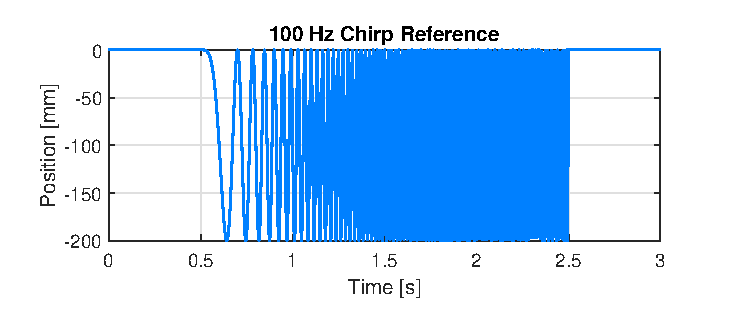
\includegraphics[width=1\linewidth]{image/ChirpRef.eps}
 	\caption{The chirp reference with the amplitude of 100 mm and a maximum frequency component of 100 Hz.}
 	\label{fig:Reference}
 	\end{center}
\end{figure}


\subsection{Simulation Setup} 
\label{sec: Simulation Setup}

\begin{figure}[t]
 	\begin{center}
 	\subfigure[]{
   		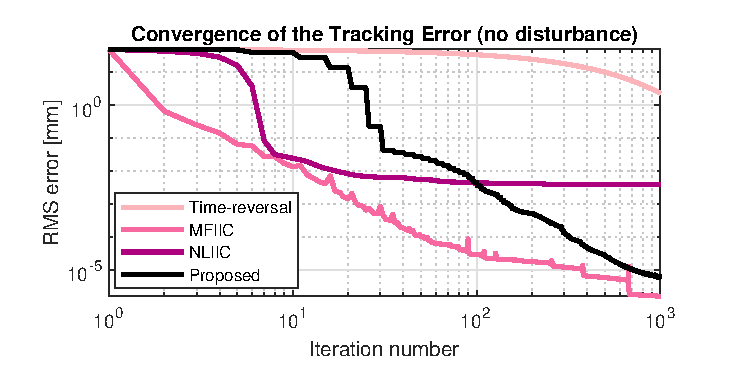
\includegraphics[width=1\linewidth] {image/ErrConvg_NoDistb.eps}
   		\label{fig:ErrConvg_NoDistb}
 	}
 	\subfigure[]{
   		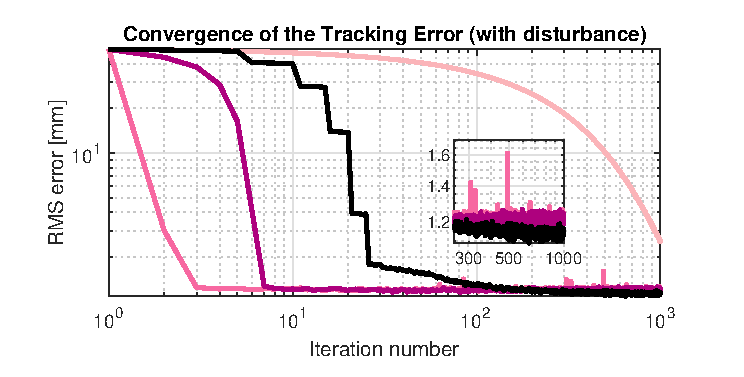
\includegraphics[width=1\linewidth] {image/ErrConvg_WithDistb.eps}
   		\label{fig:ErrConvg_WithDistb}
 	}
 	\caption{The convergence of the ILC tracking error. (a) The case with no output disturbance. (b)The case with the output disturbance $d(k)\in \mathit{N}(0,1)$.}
 	\label{fig:ErrConvg}
 	\end{center}
\end{figure}


To verify the effectiveness of the proposed algorithm, a numerical example of the system $G(z)$ is performed. As mentioned previously, $G(z)$ is pre-stabilized with the closed-loop feedback control structure. For example, assume the plant $P(z)$ is stabilized with the feedback controller $C(z)$ at sampling frequency 1 kHz, where:
\begin{align}
P(z)=\frac{0.01(z-0.9)}{(z-1)^2}; C(z)=\frac{(20z-19.9)}{z}
\end{align}  
then the system applied in the simulation $G(z)$ is
\begin{align}
G(z)=\frac{C(z)P(z)}{1+C(z)P(z)}
\end{align}


The chirp signal (linear swept-frequency cosine) is chosen as the reference trajectory in the simulation. Here the chirp trajectory with the amplitude of 100 mm and a maximum frequency component of 100 Hz is applied as the illustrated example in this paper, as shown in Fig. \ref{fig:Reference}. Note that to reduce the influence of the frequency leakage as pointed out in Sec. \ref{sec:2}, the chirp reference is padded with sufficient long zeros on the both ends.
  
To compare the performance of each model-free ILC, there are 4 cases are performed, each case is performed the updating law for 1000 iterations, and all the initial control inputs are set as $u_0(k)=r(k)$. The first case is to conduct the time-reversal based ILC, where $L_0(z)=\alpha G^{*}(z)$, $\alpha=0.1$ is chosen; the second case is to conduct the MFIIC; the third case is to apply the NLIIC [\cite{de2019data}] to enhance the robustness of MFIIC; and the fourth case is to perform the proposed algorithm, where the initial learning filter $L_0(z)$ is same as the case 1, and the updating period $n=5$, i.e., the acceleration updating occurs at 5th, 10th,..., 1000th iterations. 

\subsection{Ideal Case Without Output Disturbance} 
\label{sec: Ideal Case Without Output Disturbance}

\begin{figure}
 	\begin{center}
   	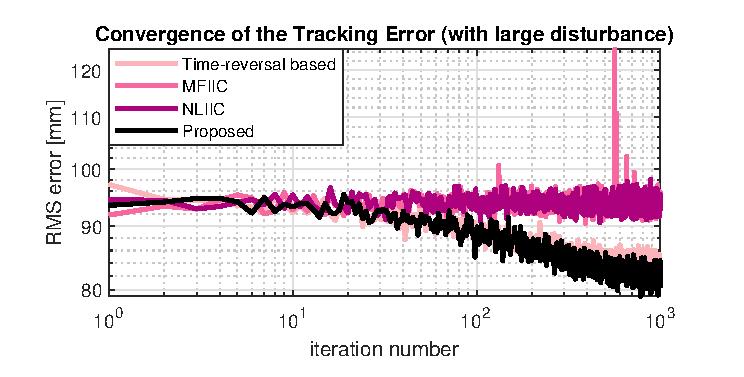
\includegraphics[width=1\linewidth] {image/ErrConvg_WithLargeDistb.eps}
 	\caption{The convergence of the ILC tracking error when the output disturbance $d(k)\in \mathit{N}(0,80)$. Both MFIIC and NLIIC do not converge.}
 	\label{fig:LargeDistb}
 	\end{center}
\end{figure}


\begin{figure}[t]
 	\begin{center}
 	\subfigure[]{
   		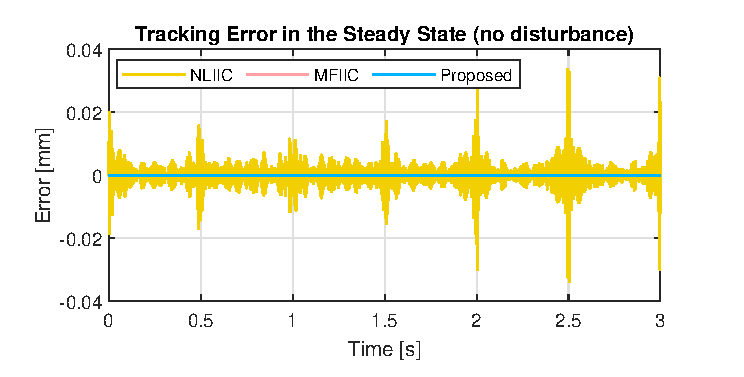
\includegraphics[width=1\linewidth] {image/TrkingErr_NoDistb.eps}
   		\label{fig:TrkingErr_NoDistb}
 	}
 	\subfigure[]{
   		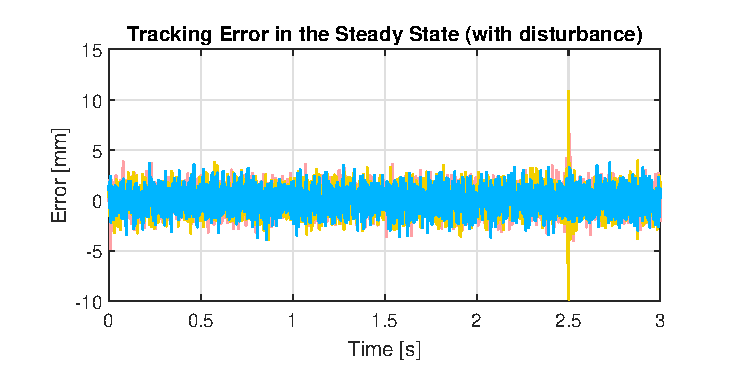
\includegraphics[width=1\linewidth] {image/TrkingErr_WithDistb.eps}
   		\label{fig:TrkingErr_WithDistb}
 	}
 	\caption{The ILC tracking error in steady-state. (a) The case with no output disturbance. (b) The case with the output disturbance $d(k)\in \mathit{N}(0,1)$. }
 	\label{fig:TrkingErr}
 	\end{center}
\end{figure}

 Consider the ideal case, where the output disturbance is neglected in this section. The only factor impacts the unideal learning for the disturbance-free case in the simulation is the frequency-leakage problem as pointed out in section \ref{sec:2}. 

Fig. \ref{fig:ErrConvg}(a) shows the error convergence of each learning law with no output disturbance. From the simulation result, it can be observed the convergence rate of time-reversal based ILC is the slowest. The convergence rate of the proposed learning law is accelerated every 5 iterations compared with time-reversal based approach, hence the learning rate is further improved. Although the convergence rate of MFIIC is faster than time-reversal based ILC, however, the unpredictable learning transient may appear in some iterations. NLIIC solve the robustness issue of MFIIC, however, the tracking is limited by the adaptive learning gain, hence the tracking performance in steady-state is much worse than MFIIC and proposed algorithm. 

On the other hand, although the convergence rate of the proposed learning law is slower than MFIIC and NLIIC, however, the learning transient is improved by avoiding the noisy signal division. Moreover, the proposed algorithm provide better tracking performance in steady-state compared to NLIIC. From Fig. \ref{fig:TrkingErr}(a), it can be observed the NLIIC is suffered from the influence of frequency leakage problem. The dual-mode learning of the proposed algorithm further reduces the tracking error caused by the frequency leakage, hence the steady-state performance is improved. The RMS error and maximum error of each learning law at the 1000th iteration with no output disturbance is shown in Table \ref{tab:TrackingError}. 

\begin{table}[t]
\begin{center}
\caption{The ILC tracking error obtained from different methods}
\label{tab:TrackingError}
\begin{tabular}{|c|rr|rr|rr|rr|}
\hline
\textbf{}  & \multicolumn{2}{c|}{\textbf{No Disturbance}}                                                                             & \multicolumn{2}{c|}{\textbf{With Disturbance}}                                                                                    \\ \cline{2-5} 
\textbf{Method} &{RMSE} &{MaxE} &{RMSE} &{MaxE} \\ 
\textbf{} & [mm] & [mm] & [mm] & [mm] \\ \hline
Time-reversal   & 2.33      & 6.13   & 2.54 & 8.15    \\
MFIIC     & 1.64e-06         & 1.75e-06      & 1.24 & 9.61     \\
NLIIC    & 0.00410      & 0.0339     & 1.22     & 13.8 \\
Proposed  & 6.25e-06        & 1.64e-05       & 1.12 & 4.52          \\ \hline
\end{tabular}
\end{center}
\end{table}

\subsection{Output Tracking with Trial-variant Disturbances} 
 \label{sec: Output Tracking with Trial-variant Disturbances}
 
 Consider the trial-variant normally distributed random time sequences (the MATLAB function: randn) are applied as the output disturbances, the tracking result of each model-free learning law is shown in this section. Note that to reduce the influence of the output disturbances in error convergence, both the NSR conditions of MFIIC and NLIIC are set as:
 \begin{align}
U_{j+1}(e^{j\omega})=\begin{cases}
 & U_{j}(e^{j\omega})+\rho_j\frac{U_j(e^{j\omega})}{Y_j(e^{j\omega})}E_j(e^{j\omega}),\\ 
 &\text{ if } |Y_j(e^{j\omega})|\neq 0 $ and $ |R(e^{j\omega})|> \delta ;\\ 
 & U_{j}(e^{j\omega});\text{ otherwise}
\end{cases}
\end{align}

Fig. \ref{fig:ErrConvg}(b) shows the error convergence of each learning law with the output disturbances, where the standard deviations of the disturbances are 1 mm and the mean values are 0 mm (i.e., $d(k)\in \mathit{N}(0,1)$). From the simulation results, it can be seen the convergence rate of the proposed algorithm is dramatically improved compared with time-reversal based ILC, and the learning transient is also reduced, hence the robustness is improved. Moreover, the tracking performance at the 1000th iteration of the proposed algorithm is supreme, as shown in the right column of the Table \ref{tab:TrackingError}. 

To show the robustness and the steady-state performance of the proposed algorithm outperforms that of the  MFIIC and NLIIC, consider the extreme situation that the output disturbances with the standard deviations of 80 mm and the mean values of 0 mm (i.e., $d(k)\in \mathit{N}(0,80)$) are applied to track the 100 mm chirp reference, as shown in Fig. \ref{fig:LargeDistb}. Although NLIIC provides a smoother learning curve than MFIIC approach, however, the tracking error doesn't converge to a lower level. On the other hand, since the proposed algorithm is based on time-reversal based ILC, the robustness and the limited steady-state tracking performance problems can be remedied. 

From Fig. \ref{fig:TrkingErr}(b), it can be observed the maximum tracking error of MFIIC and NLIIC occur at around 2.5 sec, i.e., the high-frequency components of the chirp reference. The proposed algorithm not only further reduces the tracking error in high-frequency, but also provides a more robust and flexible updating law compared with MFIIC and NLIIC, hence the tracking performance is improved if the output disturbances are considered.


\chapter{Case Study 1: Triangular Wave Tracking of Galvo Scanner}
\label{ch: Case Study 1: Triangular Wave Tracking of Galvo Scanner}


\section{System Overview} 
 \label{sec: System Overview}


\begin{figure}
 	\begin{center}
   	\includegraphics[width=1.3\linewidth] {image/Galvo_Scanner_SysOverview}
 	\caption{The schematic diagram of the galvo scanner system.}
 	\label{fig:Galvo_SysOverview}
 	\end{center}
\end{figure}



\section{Repetitive Controller Design} 
 \label{sec: Repetitive Controller Design}
 
 
\section{Experiment Setup} 
 \label{sec: Experiment Setup}
 
 
\section{Experiment Result} 
 \label{sec: Experiment Result}

%------------------------------------
% Thesis Body -- end
%------------------------------------

\bibliographystyle{IEEEtran}
\bibliography{thesis}
\end{document}
